% !TEX root = main.tex

\pagebreak
\section{Methodology}
\label{sec:methodology}

In this section, we detail the experimental methodology designed to evaluate the Ceph file system for \ac{HPC} environments. A specialized approach was necessary due to the unique requirements and constraints of \ac{HPC} environments. These include factors such as the lack of root privileges on standard \ac{HPC} compute nodes, dynamic allocation of compute resources, as well as our requirement to isolate hardware performance. Consequently, the primary goals of the methodology detailed in this section are as follows:

\begin{itemize}
    \item To engineer an automated deployment framework capable of rootless provisioning of Ceph clusters, integrating with standard \ac{HPC} cluster nodes, workload managers such as Slurm, and rootless \acs{HPC}-optimized container runtimes, such as Apptainer.
    \item To eliminate bandwidth and latency limitations of physical hard disks from performance measurements through the use of Ceph's memory backed storage backend, allowing for our evaluation to focus on Ceph's internal abstraction layers.
    \item To establish a tuned baseline for network communication performance over common \ac{HPC} fabrics---specifically, the Omni-Path and InfiniBand fabrics available on the \acs{GWDG} cluster---in order to potentially attribute possible performance bottlenecks which arise to Ceph's reliance on the \ac{TCP/IP} stack for its communication.
    \item To construct a performance testing pipeline using \ac{HPC} \acs{I/O} performance benchmarking tools such as \ac{IOR} and mdtest, which test multiple \ac{I/O} access patterns common in \ac{HPC} at various scaling levels.
    \item To establish a secondary Ceph cluster with tightly-controlled performance parameters, in order to evaluate the system administration and theoretical performance scaling aspects of the file system.
\end{itemize}

The subsections which follow describe our evaluation of existing cluster deployment tools, our custom Ceph deployment system, network tuning, and our benchmarking framework.

\subsection{Deployment Tools}

Ceph clusters can be deployed using a variety of standard tools. However,
several challenges were presented when attempting to implement these in the
\ac{HPC} test environments that were available for this thesis. We will
initially cover existing tools for production deployments, followed by the
deployment tool created for this thesis.

\subsubsection{Cephadm}
\label{sec:cephadm}

Cephadm is a first-party orchestration tool designed for the deployment of Ceph clusters. It manages cluster deployment by performing setup operations such as storage provisioning and placement of daemons on participating cluster nodes. It is generally the recommended tool for the deployment of production-ready Ceph clusters\footnote{\url{https://docs.ceph.com/en/latest/install/}. Accessed 21.01.2026.}.

The Cephadm orchestrator requires root permissions in order to perform operations such as storage configuration, as well as an interface to either Docker or Podman as a container runtime, used to create daemon containers. The hardware available for this thesis, standard \ac{HPC} cluster nodes, neither allowed for root access nor access to a fully-featured Podman or Docker installation. Instead, only the Apptainer container runtime was provided.

In addition, modern Ceph versions use the BlueStore storage backend, which performs read/write operations directly on block devices (i.e., physical disks, partitions, or logical volumes) rather than using an intermediate file system. This requires both the hardware (i.e., the disks themselves to be available), as well as the permissions necessary to read and write to them. Both of these options were not available on the \ac{HPC} cluster. While the legacy FileStore backend could have theoretically been run rootless, we do not consider the data gathered from this backend to be useful for evaluation. This is primarily due to the fact that, since January 2025, the last Ceph version with support for the FileStore Backend (17, Quincy) is unsupported\footnote{\url{https://docs.ceph.com/en/latest/releases/\#active-releases}. Accessed 02.02.2026.}.

The cephadm utility will still be used in this thesis to evaluate the
system administration aspect of the file system. However, because the hardware available for this purpose consists of a single performance- and network-limited computer, large-scale stress testing will not be performed on the Cephadm-deployed cluster. This deployment is referred to as the
\enquote{Production Deployment} and detailed further in~\cref{sec:production-deployment}.

\subsubsection{Alternatives}

Other orchestration tools, such as Rook, have similar requirements which complicate deployment on the \ac{HPC} cluster. Due to the aforementioned permission limitations and the desire to eliminate sources of variance outside of Ceph's direct control as much as possible, such as variations in \ac{SSD} performance, a custom deployment and benchmarking method was implemented in this thesis.

\subsection{Custom Deployment}
\label{sec:custom-deployment}

Due to the unique limitations of the cluster, as well as the time-consuming and therefore impractical nature of deploying several different cluster configurations manually, a custom deployment tool was created in this thesis in order to deploy and benchmark Ceph clusters of various sizes as well as under various client workloads. The tool has been named \enquote{Cuttlefish} and will be referred to as such in the following sections.

Cuttlefish is built for Ceph cluster deployment taking into account the limitations of the \ac{HPC} cluster. Specifically, it must function under the following constraints:

\begin{itemize}
    \item Elevated privileges are not required on any node in the cluster.
    \item Daemons must run either without a container engine, or on Apptainer, the latter of which was available on the test nodes.
    \item The number of daemons of each type as well as the distribution should be configurable.
    \item The orchestrator should be capable of deploying daemons on dynamically allocated nodes, which have varying \ac{IP} addresses and may not be pre-configured.
\end{itemize}

Cuttlefish is built to work with Apptainer and Slurm. Slurm is used for the allocation of nodes from the \ac{HPC} cluster pool, and Apptainer is used to run the daemons in containers regardless of the host operating system. The latter is similar to the method used by Cephadm, although the container runtime is different.

Due to the BlueStore backend's reliance on direct disk access, it is not possible to run large-scale BlueStore tests on the \ac{HPC} cluster without root permissions. However, Ceph provides a memory-backed storage backend. This backend, known as MemStore, is designed primarily for testing purposes, and does not require elevated privileges---objects are stored in \ac{RAM}. For the purposes of these benchmarks, this backend is sufficient, as the goal of our benchmarking process is to identify bottlenecks within Ceph itself, rather than the limitations of the underlying disks. Being an in-memory storage backend, MemStore is less likely to be a bottleneck due to the higher bandwidth and lower latency provided by \ac{RAM}. Given that the memory bandwidth is significantly higher than the network bandwidth, we assume that the network becomes a performance bottleneck before memory does. To validate this, prior to running benchmarks, the memory bandwidth of the system will be tested using the Intel Memory Latency Checker\footnote{\url{https://www.intel.com/content/www/us/en/download/736633/intel-memory-latency-checker-intel-mlc.html}. Accessed 26.02.2026.} (mlc), or pmbw\footnote{\url{https://panthema.net/2013/pmbw/}. Accessed 26.02.2026.} if mlc is not capable of running due to system constraints.

A summary of the communication between the various involved systems is summarized in \Cref{fig:cuttlefish_deployment_seq_diagram} as a sequence diagram. Additionally, we will use an example cluster to demonstrate how the system state is modified by the various steps in the deployment process, shown in~\cref{tab:example-cluster-layout}.

\begin{table}[h]
    \centering
    \begin{tabular}{|ccccccc|}
        \hline
        Hostname & IP Address & \acs{RAM} & Monitors & Managers & \acp{MDS} & \acp{OSD} \\
        \hline
        node1    & 192.0.2.1 & \multirow{4}{*}{256 GiB} & 1        & 1        & 1         & ---       \\
        node2    & 192.0.2.2 & & ---      & ---      & ---       & 3         \\
        node3    & 192.0.2.3 & & ---      & ---      & ---       & 4         \\
        node4    & 192.0.2.4 & & ---      & ---      & ---       & 3         \\
        \hline
    \end{tabular}
    \caption[Example Cluster Layout]{An example cluster layout which will be used for demonstration purposes.}
    \label{tab:example-cluster-layout}
\end{table}

\begin{figure}[htbp]
    \centering
    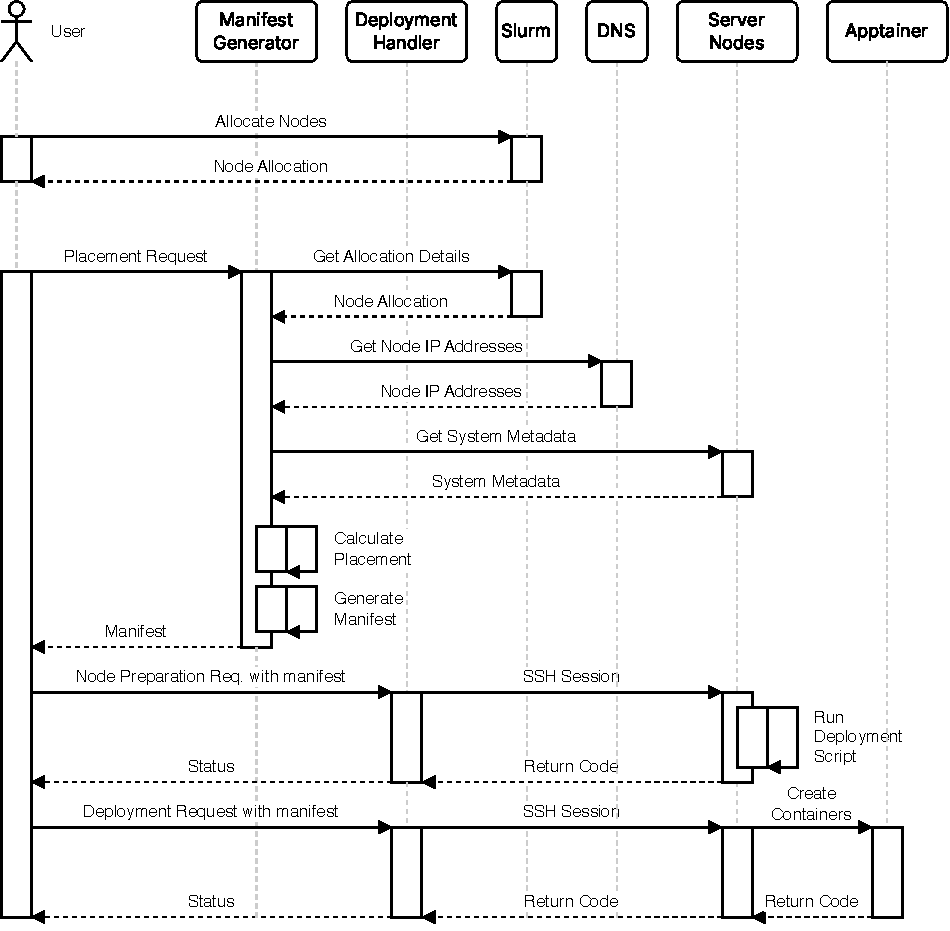
\includegraphics[width=\linewidth]{assets/cuttlefish/deployment_seq_diagram.pdf}
    \caption[Cluster deployment sequence diagram]{
Sequence diagram for the cluster deployment process. The deployment scripts
(manifest generator and deployment handler) communicate with external services
in order to generate a manifest containing all necessary details to start the
cluster. With the complete manifest, the deployment handler communicates with
participating nodes and their container runtimes to bring up the requested
daemons.
}
    \label{fig:cuttlefish_deployment_seq_diagram}
\end{figure}

\subsubsection{One-Time Operations}

Certain operations within the deployment must only be performed once and can be reused across an unlimited number of cluster deployment and teardown cycles.

Ceph daemons and clients communicate with each other using an encrypted protocol known as cephx\footnote{\url{https://docs.ceph.com/en/tentacle/dev/cephx/}. Accessed 20.01.2026.}. Monitor nodes contain the keys of all nodes, including their own key shared across the monitors, while individual daemon types only have their own keys. The keyring then contains the keys as well as the allowed permissions: an example of a keyring file can be found in~\cref{appendix:sample-ceph-keyring}.

Access to a Ceph cluster is not required for this step, only the command line tools which are available in the upstream Ceph container image. Cuttlefish includes a tool which generates this keyring file once, with configurable permissions. This keyring file is then used and preserved across different deployments and reconfigurations. For example, the keyring can contain keys for 512 \acp{OSD} and 10 monitors, even if the deployed cluster never contains this many daemons. The rest of the keys in the keyring are simply ignored until more daemons are created.

\subsubsection{Node Allocation \& Placement}
\label{sec:node-allocation-placement}

The nodes available for testing during this thesis were part of the regular production compute cluster at the \ac{GWDG}. Nodes are allocated on-demand, and change depending on node availability. Therefore, a request to allocate e.g., 16 nodes on a cluster may return a different set of nodes depending on the nodes used by other users' jobs. A job was first allocated using the \texttt{salloc} command, which creates a node allocation for the cluster deployment system to use. \Cref{lst:slurmalloc} shows a typical distribution of nodes after an allocation is granted, gathered using \texttt{squeue}\footnote{Output from \texttt{squeue -{}-me} formatted to remove unnecessary/internal information.}.

\lstinputlisting[
    caption={
        [Slurm Node Allocation]
        A typical Slurm node allocation performed on the \ac{GWDG} compute cluster's 
        \texttt{medium96s} partition, containing a set of nodes ready for use.
    },
    label={lst:slurmalloc},
    frame=single,
    breaklines=true
]{assets/cluster/squeue-me.txt}

Due to the dynamic nature of the allocations, we automate the mapping of Ceph daemons onto nodes. The user may specify the desired state of the cluster at a high level, and the placement will be performed according to the user's instructions. The placement algorithm allows for the following requirements and constraints to be taken into consideration:

\begin{itemize}
    \item Total number and type of daemons (e.g., 1 monitor, 1 \ac{MDS}, 8 \acp{OSD})
    \item Number of nodes to use from the Slurm allocation
    \item Adjustment of constraints per daemon type
    \begin{itemize}
        \item Density: the maximum number of daemons of this type to place on a node
        \item Allowed overlaps: if no free nodes are available, allow placement on an already occupied node
        \item Disallowed overlaps: do not allow the co-location of this daemon on a node with specific daemon types (e.g., monitor and \ac{OSD} must not overlap)
        \item Required overlaps: require that the daemon be placed with another daemon of the specified type
    \end{itemize}
    \item Placement type
    \begin{itemize}
        \item Spread (S): Place daemons on the least loaded nodes
        \item Group (G): Group daemons on the most loaded node up to the density limit before considering other nodes
    \end{itemize}
\end{itemize}

The default placement policy is shown in~\cref{tbl:allowed-daemon-overlaps}.

\newcommand{\YesMark}{%
  \tikz\fill (0,0) rectangle (1.2ex,1.2ex);%
}
\newcommand{\NoMark}{%
  \tikz\draw (0,0) rectangle (1.2ex,1.2ex);%
}
\newcommand{\RequiredMark}{%
  \tikz\fill
    (0,0) --
    (1.2ex,0) --
    (0.6ex,1.2ex) --
    cycle;%
}

\begin{table}[h]
    \begin{center}
        \begin{tabular}{|cc|lcccc|}
            \hline
            \rotatebox{90}{Placement~} & \rotatebox{90}{Density~} & & \rotatebox{90}{Monitor~} & \rotatebox{90}{Manager~} & \rotatebox{90}{\acs{MDS}~} & \rotatebox{90}{\acs{OSD}~} \\
            \hline
            Spread & 1 & Monitor & \NoMark  & \YesMark & \YesMark & \NoMark \\
            Spread & 1 & Manager & \RequiredMark & \NoMark  & \YesMark & \NoMark  \\
            Spread & 128 & \acs{MDS} & \YesMark & \YesMark & \YesMark & \NoMark \\
            Spread & 128 & \acs{OSD} & \NoMark  & \NoMark  & \NoMark  & \YesMark \\
            \hline
        \end{tabular}
    \end{center}
    \begin{center}
        \begin{tabular}{ccccccc}
             Overlaps: & \NoMark & Disallowed & \YesMark & Allowed & \RequiredMark & Required \\
        \end{tabular}
    \end{center}
    \caption[Default Placement Policy]{The default daemon placement policy. The daemon types on the left represent the daemon to be placed, and the daemon types in the table header represent the existing daemons on the node.}
    \label{tbl:allowed-daemon-overlaps}
\end{table}

\subsubsection{Ceph Autoconfiguration}
\label{sec:ceph-autoconfig}

The template Ceph configuration is similar to that of a regular Ceph cluster: it contains the startup configuration shared across all nodes. However, in addition to the template itself, additional fields are added to the final configuration in order to allow for the cluster layout to change while keeping the template configuration static. \Cref{lst:ceph-conf} shows an example of a minimal ceph.conf which contains a configuration for a Ceph cluster with MemStore \acp{OSD}.

\lstinputlisting[
    language=ini,
    caption={
    [Minimal Ceph Configuration]
    Minimal configuration file used for bootstrapping the Ceph cluster, allowing for
    options to be changed by the user manually prior to the bring-up of the cluster.
    For instance, the default minimum pool size is reduced to 1 for testing purposes.
    },
    label={lst:ceph-conf},
    frame=single,
    breaklines=true
]{assets/cuttlefish/example.ceph.conf}

Ceph daemons require the location of monitor nodes to be defined in the configuration. Instead of being hardcoded into the configuration, the monitor node list is generated dynamically based on the node allocation and placement policy as described in~\cref{sec:node-allocation-placement}. Once daemons have been allocated to nodes, the \ac{IP} addresses of the nodes containing monitor daemons are gathered and used to populate the monitor configuration.

The amount of memory allocated to each \ac{OSD} is also selected based on the maximum number of \acp{OSD} per node within the cluster as well as the available memory. The memory limit is manually set: for benchmarking purposes, we have targeted 75\% of the available memory on the node. The remaining 25\% is reserved for the operating system, background tasks, and Ceph daemon process overhead. Each \ac{OSD} process requires additional memory beyond its MemStore allocation to operate, as do other services, such as monitors and \ac{MDS} daemons, and we observed that the maximum memory usage of the daemons was well within the remaining 25\% on our 256\,GiB and 512\,GiB nodes.

For our example cluster (see~\cref{tab:example-cluster-layout}), this results in \texttt{node1} being added to the monitor configuration and a memory target based on the most loaded node with 4 \acp{OSD} and a memory target of 192 GiB across 4 \acp{OSD} for 48 GiB per \ac{OSD}, or 51,539,607,552 bytes when converted. These lines are created as shown in~\cref{lst:ceph-conf-dynamic}, and appended to the base Ceph configuration from~\cref{lst:ceph-conf}. Note that~\cref{lst:ceph-conf-dynamic} only shows the added values, not the entire configuration.

\lstinputlisting[
    language=ini,
    caption={
    [Dynamically Generated Ceph Configuration Items]
    Dynamically generated Ceph configuration items, created based on the 
    available cluster resources and user-specified targets.
    },
    label={lst:ceph-conf-dynamic},
    frame=single,
    breaklines=true
]{assets/cuttlefish/dynamic.ceph.conf}

\subsubsection{Container Image}

The image to use for deployment can be specified in the configuration. For instance, it is possible to use the default upstream Ceph image or a custom-built image. For the benchmarks, the official Ceph Tentacle release (v20.2.0) image is used\footnote{The official image is available at \url{https://quay.io/repository/ceph/ceph}. Accessed 04.01.2026.}.

Due to the fact that the \ac{HPC} cluster only provides Apptainer as a container runtime, the images are converted from the original \ac{OCI} format used by Docker and Podman into the Apptainer image format, known as \ac{SIF}\footnote{Apptainer was formerly known as Singularity, hence the name.}.  This functionality is performed natively by Apptainer by prepending \texttt{docker://} to the image name, enabling its compatibility mode.

\subsubsection{Initial Configuration}

\lstinputlisting[
    language=ini,
    caption={
    [Generated Cluster Manifest]{
        A manifest produced by the manifest generator for the example
        cluster~(cf.~\cref{tab:example-cluster-layout}), containing 
        monitors, \acp{OSD}, and \acp{MDS}.}
    },
    label={lst:cuttlefish-manifest},
    frame=single,
    breaklines=true,
    float
]{assets/cuttlefish/example.manifest.json}

The manifest generator combines all of the required information from user configurations and external systems in order to build a complete cluster manifest. This manifest contains all of the information necessary to build a Ceph cluster, taking into consideration the required resources and available nodes. In addition, the Ceph configuration is also modified to add configuration details which change when the cluster changes---namely, the list of monitor nodes, which is allocated dynamically by the deployment script. For the cluster layout in~\cref{tab:example-cluster-layout}, the manifest would be generated as shown in~\cref{lst:cuttlefish-manifest}. This ensures that all daemons which are deployed using the manifest can communicate correctly without additional manual configuration steps.

\subsubsection{Preparation of Cluster Nodes}

In order to prepare the cluster nodes for running Ceph daemons, the dynamically allocated compute nodes must be brought to a state such that they are ready to run the orchestration stack and Ceph containers. Because we use node-local storage for our deployment, the \ac{HPC} cluster nodes are not pre-configured with the required folder structure and software dependencies.

The initial step of the preparation involves retrieving the node list from Slurm. The system queries Slurm, searching for a user-specified job name (by default cuttlefish). Once this job is found, the list of candidates for placement is gathered. The hostnames are initially gathered through Slurm, while additional details, such as the list of interfaces and network addresses, are gathered via \ac{SSH}. On the \ac{GWDG} cluster, the hostname provided by Slurm can be used with \ac{SSH} in order to connect to the cluster nodes with passwordless host-based authentication, as long as the job is running and the job's user matches the current user.

Next, the orchestrator connects to all cluster nodes via \ac{SSH}, in order to bootstrap a new Python virtual environment on local storage. The package sources themselves are stored on shared cluster storage. However, for performance reasons, the dependencies and the Cuttlefish orchestration package itself is installed on local storage, primarily in order to improve startup times. It also allows for nodes with potentially different processor configurations to be supported, although we only use nodes with identical hardware configurations in this thesis.

Once all nodes complete this setup phase, the cluster is ready for the deployment phase.

\subsubsection{Deployment}

Once all of the previously discussed prerequisites are fulfilled, the deployment of the cluster can be performed. The deployment controller script establishes \ac{SSH} connections to nodes which are part of the cluster, executing the deployment worker script on the nodes in order to bring the cluster to the user's desired state.

The deployment worker compares its current state to that of the manifest and starts Apptainer instances as necessary. Apptainer instances are the closest equivalent to standard containers in Docker or Podman; instances are designed for long-running applications and services. The following steps are performed to bring up Ceph daemons:

\begin{itemize}
    \item The basic file structure is generated in a temporary directory, with the layout shown in~\cref{fig:daemon-file-folder-layout}.

    \begin{figure}[h]
        \centering
        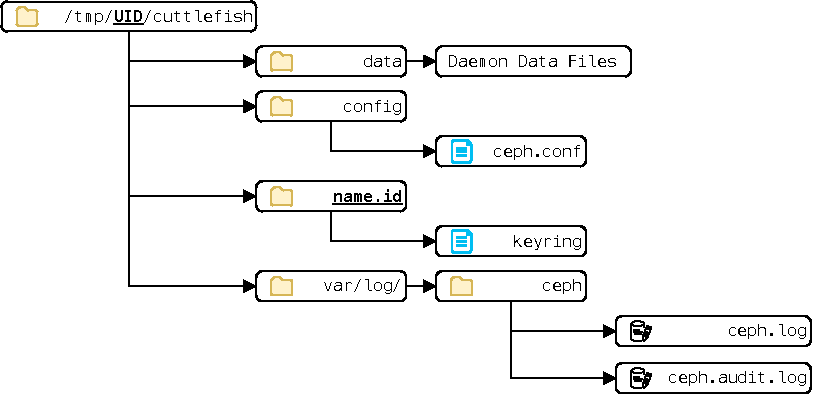
\includegraphics[width=\linewidth]{assets/cuttlefish/file_folder_layout.pdf}
        \caption[Daemon File/Folder Layout]{File and folder layout of a daemon deployed using Cuttlefish. The \texttt{ceph.conf} file is shared across all daemons, while the keyring is generated per-daemon from the full keyring stored in the manifest. The data folder contains data generated and/or required by Ceph for that specific daemon. Monitors write to the \texttt{ceph.log} and \texttt{ceph.audit.log} files.}
        \label{fig:daemon-file-folder-layout}
    \end{figure}
    
    \item The configuration is extracted from the manifest and written to \texttt{config/ceph.conf}, used by all nodes.
    \item The keyring is extracted from the manifest, and only the key for the daemon is placed in the daemon's folder, e.g., \texttt{osd.0/keyring}. For monitors, the entire keyring with the pre-generated keys for all daemons is provided, even if only a subset of daemons defined in the keyring are deployed.
    \item Monitors and \acp{OSD} are initialized if their data directories are empty with the \texttt{-{}-mkfs} commands for each daemon.
    \item Daemons are started in the order of: monitors, managers, \acp{OSD}, \acp{MDS}, followed by other daemons (if any) as Apptainer instances with the appropriate folders mounted.
\end{itemize}

After these steps are completed, each node will run its assigned daemons within independent Apptainer instances. An example is shown in \Cref{lst:apptainer_instance_list}, shortened for brevity.

\lstinputlisting[
    caption={Apptainer Instance Listing for Running Cluster},
    label={lst:apptainer_instance_list},
    frame=single,
    breaklines=true
]{assets/cuttlefish/apptainer_instance_list.txt}

To confirm that all instances are running, the layout of running instances can be requested from the deployment script, as shown in \Cref{lst:daemon_get_state}. This must be performed from a machine with \ac{SSH} access to and login permissions for the member nodes.

\lstinputlisting[
    caption={Listing of Running Daemons},
    label={lst:daemon_get_state},
    frame=single,
    breaklines=true
]{assets/cuttlefish/daemon_get_state.txt}

\subsubsection{Teardown}

Teardown follows the same process as deployment, using the deployment controller
script with the command shown in~\cref{lst:daemon-teardown}.

\lstinputlisting[
    caption={[Cluster Teardown]{Command used to tear down a Ceph cluster. This command stops all Ceph daemon containers as defined in the manifest, followed by the deletion of the folder structure generated in~\cref{fig:daemon-file-folder-layout}.}},
    label={lst:daemon-teardown},
    frame=single,
    breaklines=true
]{assets/cuttlefish/teardown.txt}

Note that this command does not cancel the Slurm job. The cluster can be re-deployed immediately: either with the same manifest, or with a manifest generated using different parameters, e.g., more \acp{OSD} or a different distribution of daemons on the cluster nodes within the allocated Slurm job.


\subsection{Production Deployment}
\label{sec:production-deployment}

In addition to Ceph performance testing, we intend to evaluate Ceph from a systems administration perspective. In order to do so, it is necessary to test Ceph's production-ready components, such as cephadm and BlueStore, to evaluate the following functionality:

\begin{itemize}
    \item Ease of deployment from scratch
    \item Processes involved in adding and removing storage from the cluster
    \item Enablement of various Ceph services
    \item Performance characteristics
\end{itemize}

Note that, unlike~\cref{sec:custom-deployment}, the performance characteristics being referred to in this section are not intended to test Ceph's performance limits, as the hardware available for this rootful production deployment is significantly more performance-limited than that available for the custom deployment. Instead, the intent is to evaluate how Ceph interacts with hardware under well-known, controlled lab conditions. To that end, we will control factors such as \ac{OSD} layout and disk \ac{I/O} performance in order to compare Ceph's theoretical behaviour with observed behaviour.

\subsubsection{Deployment Hardware}

The deployment consists of a test cluster with 8 nodes, which are configured as
virtual machines on a single host, shown in~\cref{tab:dev-cluster}.

\begin{table}[h!]
    \centering
    \begin{tabular}{|ll|}
        % \multicolumn{2}{Host Hardware} \\
        \hline
        \multicolumn{2}{|l|}{\textbf{Host Details}} \\
        \hline
        Host \ac{OS}        & Cent\acs{OS} Stream 9 \\
        \ac{CPU}            & Intel Xeon E5-1650 v3 (6 cores, 12 threads) \\
        \ac{RAM}            & 256 GiB \\
        Disk                & 2x 480 GB \acs{RAID} 0 \ac{SSD} \\
        Ceph vDisk Storage  & 128 GiB \texttt{tmpfs} \\
        \hline
        % \multicolumn{2}{Guest Hardware}
        \multicolumn{2}{|l|}{\textbf{Guest Details}} \\
        \hline
        Hypervisor          & Linux KVM via libvirt \\
        Hostnames           & cvm[1-8] \\
        \acs{IP} Addresses  & 10.1.1.[1-8] \\
        v\acs{CPU}s         & 4 (2 cores, 4 threads) \\
        \acs{RAM}           & 16 GiB \\
        Boot Disk           & 100 GiB Virt\acs{IO} Block \\
        Ceph vDisk          & 16 GiB Virt\acs{IO} Block on \acs{RAM}-backed tmpfs \\
        Guest \acs{OS}      & Cent\acs{OS} Stream 9 \\
        Networking          & Virt\acs{IO} \\
        \hline
    \end{tabular}
    \caption[Development Cluster Hardware]{The development cluster used for system evaluation and lab-controlled performance testing.}
    \label{tab:dev-cluster}
\end{table}

\subsubsection{Performance Throttling}

We will primarily be evaluating how well Ceph performs with a known upper limit to disk performance. Libvirt supports setting \ac{I/O} limits per disk based on user-specified \ac{IOPS} or bandwidth targets, as well as other, more granular options as shown in~\cref{lst:blkdeviotune}.

\lstinputlisting[
    caption={
        [VirtIO Block Device Throttling]
        Available options for the \texttt{virsh blkdeviotune} command for throttling disk performance.
    },
    label={lst:blkdeviotune},
    frame=single,
    breaklines=true
]{assets/virt/blkdeviotune.txt}

The throttling can be validated in the virtual machines by running a tool such
as hdparm or \ac{FIO}, as shown in~\cref{lst:hdparm-fio-throttling}.

\lstinputlisting[
    caption={
        [Throttling Validation with fio/hdparm]
        Validation of a read limit of 50 MiB/s ($\approx$52.43 MB/s), performed with fio and hdparm. Only the summary is shown in the fio output for clarity.
    },
    label={lst:hdparm-fio-throttling},
    frame=single,
    breaklines=true
]{assets/virt/fio-check-speed.txt}

\subsection{Network Optimization}

The performance of any networked file system is fundamentally limited by the underlying network on which the file system communicates. The network's characteristics, such as latency and throughput, impose a theoretical upper bound on the file system's capabilities. To distinguish between the limitations imposed by Ceph's architecture and that of the network hardware, this section establishes our methodology for tuning network performance and establishing a throughput baseline.

Ceph deployments do not utilize \ac{RDMA} by default for communication, in contrast to \acs{HPC}-native file systems such as Lustre and BeeGFS. While \ac{RDMA} is a common feature in \ac{HPC} networking hardware, Ceph relies on the standard \ac{TCP/IP} stack for its communication. The use of \ac{TCP/IP} over \ac{RDMA} introduces several performance trade-offs~\cite{linux_kernel_networking}:

\begin{itemize}
    \item \ac{TCP/IP} processing is primarily performed in software, incurring significant performance costs at high throughputs through packet processing and context switching overhead.
    \item \ac{RDMA} performs zero-copy transfers, which allow for direct placement of data from the network adapter to application memory. However, \ac{TCP/IP} performs multiple buffer copies throughout the networking stack before reaching user space, incurring additional overhead.
    \item The aforementioned kernel overhead and memory copies lead to increased \ac{CPU} usage, reducing the compute performance available for \ac{HPC} workloads.
\end{itemize}

Consequently, Ceph incurs a \ac{CPU} utilization and network throughput disadvantage compared to \ac{HPC} file system competitors, inherent to its use of \ac{TCP/IP} for communication. Additionally, the modeling of \ac{TCP} performance can be more complex, as it depends on several additional factors beyond theoretical link speed:

\begin{itemize}
    \item Network type (Ethernet, InfiniBand, etc.)
    \item Kernel version and driver version, since newer kernels may have more optimized networking code
    \item Performance of the \ac{CPU}, including factors such as its clock speed, core count, memory layout, and internal interconnect bandwidth
    \item The offloads available and used on the network adapter
    \item Tunable parameters, such as:
    \begin{itemize}
        \item \ac{MTU}
        \item Congestion control algorithms
        \item Interrupt handling and steering
        \item Message buffer sizes
    \end{itemize}
\end{itemize}

While these factors can also affect \ac{RDMA} transports, the offloading of data transport operations to network hardware mitigates much of the performance variability which can arise from host-side bottlenecks. Therefore, in the context of this thesis, the performance baselines established are intended for comparative measurements on identical hardware, rather than an absolute metric for peak performance. The following subsections cover the optimizations applied to Omni-Path and InfiniBand, as these interconnects are used in the \ac{GWDG} \ac{HPC} cluster nodes.

\subsection{Omni-Path Optimizations}
\label{sec:opa-optimization}

The majority of the production nodes used in the \ac{HPC} cluster of the \ac{GWDG} are
equipped with Omni-Path networking, and a small number with InfiniBand
networking. However, we will focus primarily on Omni-Path, as it exhibited
architectural limitations which had a significant negative impact on the
\ac{TCP} performance available over the transport. We will focus on
the configuration and issues which were particularly impactful.

Initial testing was performed on the default Omni-Path configuration on the
\ac{GWDG} computing center. The results from these tests were poor, with 
inconsistent \ac{TCP} throughput of under 20 Gbps. The configuration and
performance results are unchanged from tests previously performed on the same
hardware~\cite{using-hpc-networks}. 

\subsubsection{Recommended Optimizations}

The Cornelis optimization guide for Omni-Path~\cite{omni-path-tuning-guide}
recommends tuning the following options in order to improve the performance of
\ac{TCP/IP} over the fabric:

\begin{itemize}
    \item Adjust the \ac{MTU} of the network interface\footnote{\cite[pp.~71--75]{omni-path-tuning-guide}}
    \item Enable \ac{GSO}\footnote{\cite[pp.~76--77]{omni-path-tuning-guide}}
    \item Enable either \ac{RPS}, or Accelerated \ac{IP} without \ac{RPS}\footnote{\cite[p.~77]{omni-path-tuning-guide}}
    \item Adjust the system \ac{TCP} parameters\footnote{\cite[p.~77]{omni-path-tuning-guide}}
    \item Enable irqbalance and adjust \ac{CPU} affinity\footnote{\cite[p.~19,~pp.~81--84]{omni-path-tuning-guide}}
    \item Enable \ac{THP}\footnote{\cite[p.~24]{omni-path-tuning-guide}}
    \item Set the \ac{IOMMU} type to pass-through mode\footnote{\cite[pp.~23--24]{omni-path-tuning-guide}}
    \item Change the \ac{CPU} performance profile to disable power saving features\footnote{\cite[pp.~19--23]{omni-path-tuning-guide}}
    \item Tune the kernel parameters \texttt{num\_sdma} and \texttt{krcvqs}\footnote{\cite[pp.~34--37,~pp.~75--76]{omni-path-tuning-guide}}
    \item Enable accelerated \ac{RDMA}\footnote{\cite[pp.~62--64]{omni-path-tuning-guide}}
    \item Tune the \texttt{ib\_ipoib} kernel module\footnote{\cite[p.~76]{omni-path-tuning-guide}}
\end{itemize}

These optimization steps were mostly applied according to the steps mentioned in
the manual. However, to preserve interoperability with the existing InfiniBand
network, it was not possible to set the \ac{MTU} larger than 4KB, and additional
issues were faced when implementing accelerated \ac{IP} support in particular.
On the Omni-Path network adapter, there are 160 available receive contexts.
These contexts are consumed by kernel, netdev, and user queues. On systems where
the number of threads nears or exceeds this limit, the number of user queues are
adjusted accordingly. However, the module does not take into account any netdev
contexts, which are required for accelerated \ac{IP} functionality. The number
of threads on the test systems (192) exceeds the context limit, which caused
accelerated \ac{IP} to fail with a message that does not directly suggest that
this system is affected, as shown in
\Cref{lst:hfi1-dmesg}.

\lstinputlisting[
    caption={hfi1 Kernel Log Output},
    label={lst:hfi1-dmesg},
    frame=single,
    breaklines=true
]{assets/network/hfi1_dmesg.txt}

After manually adjusting the value for \texttt{num\_user\_contexts} to a lower
value, the netdev contexts were allocated correctly. After applying the steps in
the guide, performance was improved. However, although the average performance
was higher, the performance results remained inconsistent. A summary of the
system configuration can be found in~\cref{tbl:opa-parameters}.

\begin{table}[h]
\centering
\begin{tabular}{ll}
\hline
\textbf{Parameter}                      & \textbf{Value} \\
\hline
\ac{MTU}                                & 4000 \\
\ac{GSO}                                & Enabled \\
Accelerated \ac{IP}                     & Enabled \\
\ac{RPS}                                & Disabled \\
\texttt{irqbalance}                     & Enabled \\
\ac{THP}                                & Always \\
\ac{CPU} Scaling Governor               & Performance \\
\hline
\textbf{Kernel Parameter}               & \textbf{Value} \\
\hline
\texttt{iommu}                          & \texttt{pt} (Passthrough) \\
\texttt{hfi1.num\_sdma}                 & 16 \\
\texttt{hfi1.num\_user\_contexts}       & 140 \\
\texttt{hfi1.krcvqs}                    & 4 \\
\texttt{ib\_ipoib.recv\_queue\_size}    & 8192 \\
\texttt{ib\_ipoib.send\_queue\_size}    & 8192 \\
\hline
\textbf{Sysctl Parameter}               & \textbf{Value} \\
\hline
\texttt{net.ipv4.tcp\_rmem}             & 16384 131072 16777216 \\
\texttt{net.ipv4.tcp\_wmem}             & 16384 16384 16777216 \\
\texttt{net.ipv4.rmem\_max}             & 16777216 \\
\texttt{net.ipv4.wmem\_max}             & 16777216 \\
\texttt{net.core.somaxconn}             & 2048 \\
\texttt{net.ipv4.tcp\_mtu\_probing}     & 1 \\
\texttt{net.core.netdev\_max\_backlog}  & 250000 \\


\hline
\end{tabular}
\caption{Configured Parameters for Omni-Path}
\label{tbl:opa-parameters}
\end{table}

\subsubsection{\acs{TCP/IP} Offload Issues} 

Similarly to InfiniBand, Omni-Path runs best on its native \ac{RDMA} capable transport, \ac{PSM}. The distinguishing factor is that, even though \ac{TCP/IP} is a \enquote{non-optimal} transport for InfiniBand, modern adapters nonetheless provide hardware offloads for it. Stateless offloads have also been the norm on Ethernet adapters to the extent that, in addition to datacenter Ethernet adapters, commodity Ethernet adapters support such offloads as well\footnote{Ethernet adapter tested: Realtek RTL8111.}.

\Cref{tbl:nic-offload} shows a summary of the supported capabilities of  selected network adapters by network type, relevant for \ac{TCP/IP}, gathered using ethtool\footnote{Omni-Path Adapter: Intel 100HFA016 / 1x100Gb, InfiniBand Adapter: ConnectX-6 MT28908 / 2x200Gb, Ethernet Adapter: ConnectX-6 Dx MT2892 / 2x25GbE ports, Commodity Ethernet Adapter: Realtek RTL8111 / 1x1GbE port}.

\begin{table}[h!]
\centering
% \resizebox{\textwidth}{!}{
\begin{tabular}{lccc}
\hline
\textbf{Offload} & 
\textbf{Omni-Path} &
\textbf{Ethernet} &
\textbf{InfiniBand}
\\
\hline
Scatter-Gather                           & \checkmark & \checkmark & \checkmark \\
Generic Segmentation (GSO)               & \checkmark & \checkmark & \checkmark \\
Generic Receive (GRO)                    & \checkmark & \checkmark & \checkmark \\
RX Checksum                              &            & \checkmark & \checkmark \\
TX Checksum                              &            & \checkmark & \checkmark \\
TCP Segmentation (TSO)                   &            & \checkmark & \checkmark \\
VLAN                                     &            & \checkmark & \checkmark \\
Receive Hashing                          &            & \checkmark & \checkmark \\
\hline
\end{tabular}
% } % resizebox
\caption{NIC Offload Capabilities}
\label{tbl:nic-offload}
\end{table}

It should be noted that \ac{GRO} and \ac{GSO} are not \enquote{offloads} in the
traditional sense. These offloads are not performed by the network adapter
hardware, but rather the kernel itself in
software~\cite{linux-doc-segmentation-offloads}. The lack of offloads results in
high \ac{CPU} overhead for packet processing, and in particular the lack of
receive hashing has a pronounced effect on the way this processing is
distributed across available cores on the system.

\subsubsection{Interrupt Handling Issues}
\label{sec:interrupt-handling-issues}

\Cref{fig:opa-irq} demonstrates the \ac{CPU} bottleneck issue during the performance testing, where one core is pinned at 100\% \acs{CPU} usage. In this specific instance, performance was highly variable, often ranging between 15-45\ Gbps. As a result, the performance of \ac{TCP} over Omni-Path is significantly lower than the network adapter's physical throughput limit of 100\ Gbps. Note that this figure only displays the 24 cores which displayed non-zero utilization; the remaining cores of the 92-core, 192-thread system were idle.

\begin{figure}[h]
    \centering
    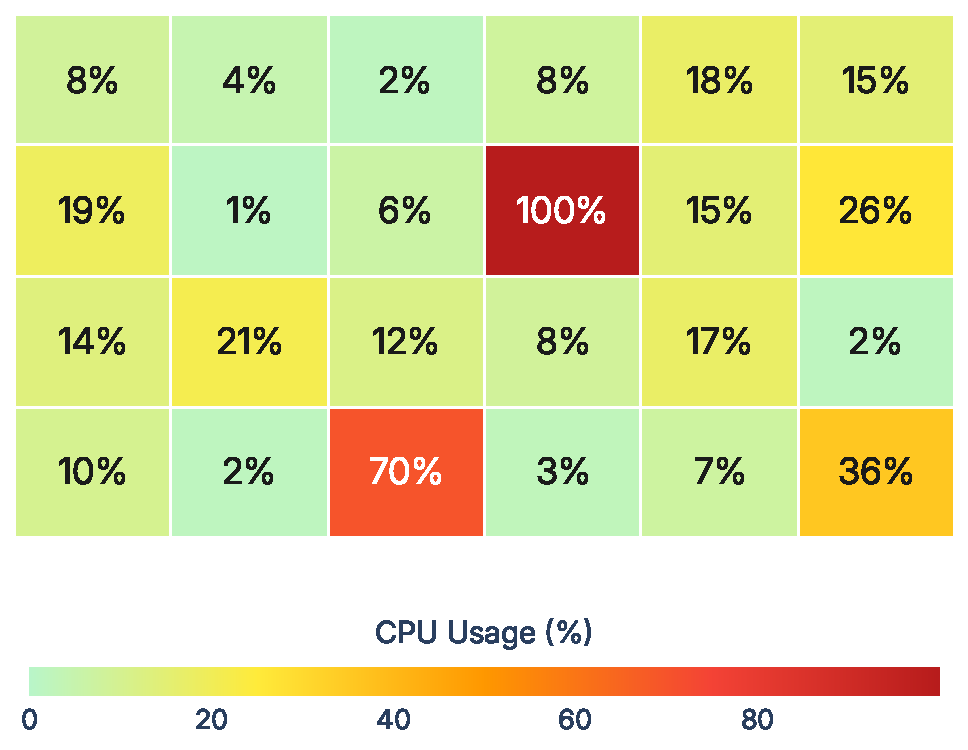
\includegraphics[width=0.5\linewidth]{assets/network/omni_path_cpu_heatmap.pdf}
    \caption[Omni-Path CPU Usage Heatmap]{Heatmap showing all cores with non-zero utilization during performance testing of Omni-Path. The heatmap demonstrates that a single core is fully loaded, while most other cores remain idle or lightly loaded.}
    \label{fig:opa-irq}
\end{figure}

The Omni-Path tuning guide also provides a method for determining the mapping of cores to interrupts~\cite{omni-path-tuning-guide}. Using this, we are able to determine which interrupt types place the most load on the \ac{CPU}. The interrupt mapping is shown in~\cref{fig:omni-path-irq-layout}.

\begin{figure}[H]
    \centering
    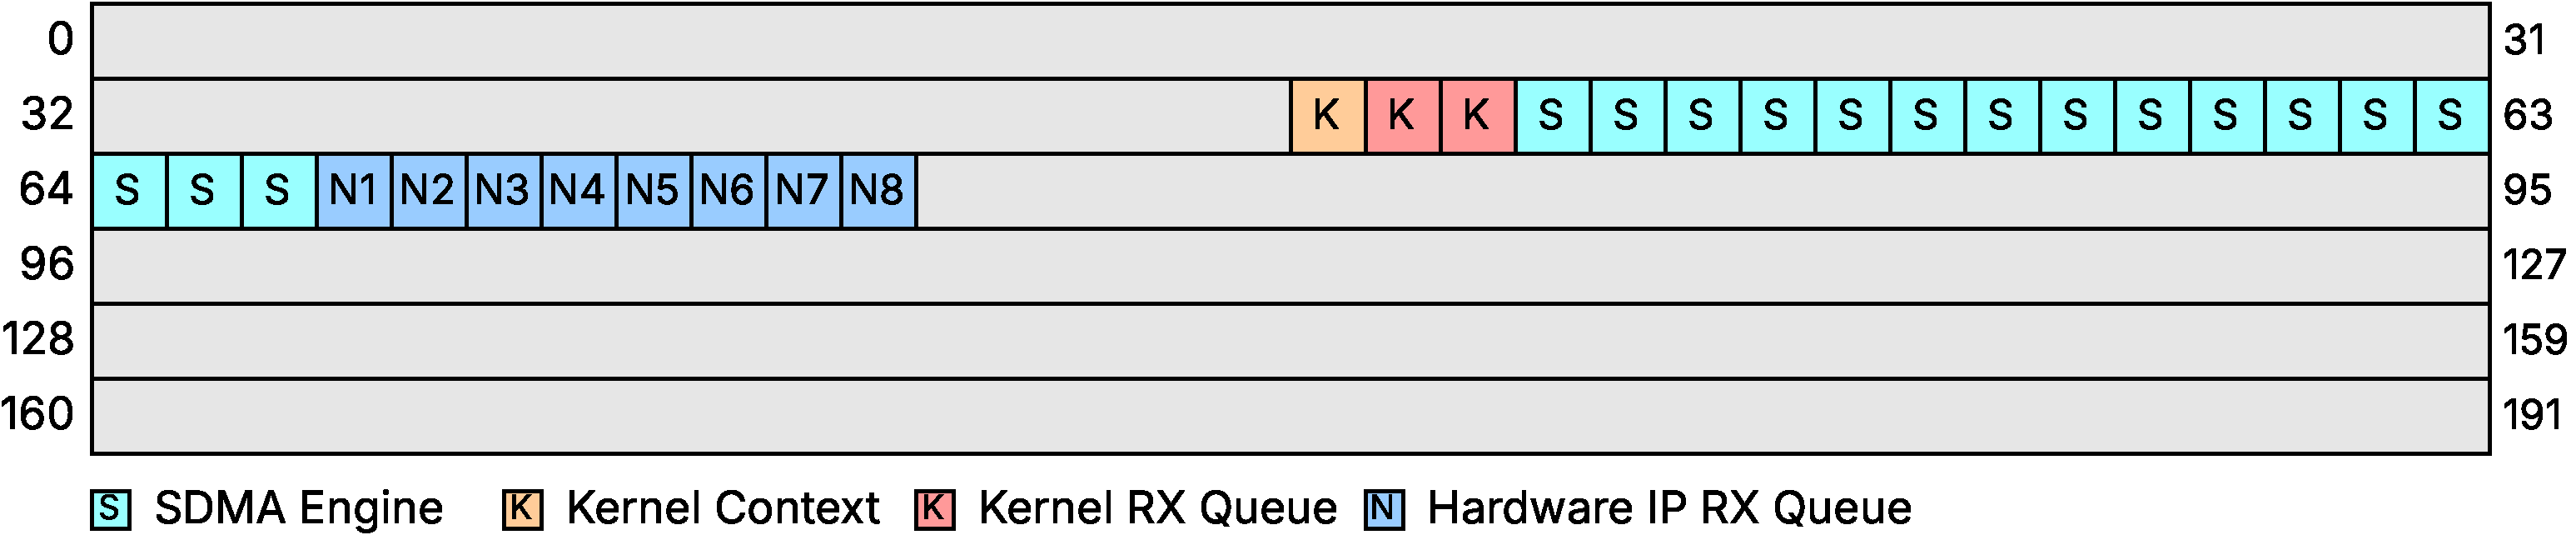
\includegraphics[width=\linewidth]{assets/network/rps/Interrupt-Layout.pdf}
    \caption{Omni-Path IRQ Layout}
    \label{fig:omni-path-irq-layout}
\end{figure}

Based on the interrupt mapping, the performance bottleneck likely stems from the \ac{CPU} usage of interrupts generated to service regular \ac{IP} traffic. This demonstrates that the processing overhead of \ac{IP} over Omni-Path is high due to the interrupt processing. More critically, despite the large number of cores---and therefore, theoretically available network processing performance---the single-core performance remains a performance bottleneck.

Beyond Ceph, these performance limitations can be of particular concern for high-bandwidth \ac{IP} traffic producers and consumers. On the \ac{GWDG} \ac{HPC} cluster, there is an additional network architecture constraint of a 4KB \ac{MTU} for interoperability with InfiniBand hardware, which further increases packet count compared to the maximum supported Omni-Path \ac{MTU} of 10KB. Furthermore, the \acp{CPU} used in the \ac{HPC} cluster are high-core-count \acp{CPU}, which generally have reduced single-core performance compared to, e.g., low-core-count consumer-grade \acp{CPU}. For instance, a consumer-grade Intel \ac{CPU} may run at 6 GHz, while a server-grade \ac{CPU} released during the same time frame may run at 4.1 GHz\footnote{Data from Intel ARK: \url{https://www.intel.com/content/www/us/en/ark.html}. Accessed 03.02 2026. Consumer \acs{CPU}: i9-14900K; Server \acs{CPU}: Xeon Gold 6538N.}.

\subsubsection{Enabling \acs{RPS} with Accelerated \acs{IP}}

The Omni-Path optimization guide recommends enabling either \ac{RPS} or
Accelerated \ac{IP} \cite[p.~77]{omni-path-tuning-guide}. However, given the
interrupt load shown in~\cref{sec:interrupt-handling-issues} as well as the
suboptimal performance, an experimental evaluation of \ac{RPS} in combination
with Accelerated \ac{IP} was performed. To that end, a specialized script was
developed to automatically assign available cores to network queues under the
following constraints:

\begin{itemize}
    \item \ac{RPS} flows can be placed on the same \ac{NUMA} node as the original interrupts to minimize latency, or spread across multiple nodes to potentially improve throughput.
    \item The number of \ac{RPS} flows, as well as the cores on which these \ac{RPS} flows are placed, are adjusted such that they do not overlap with existing interrupts.
    \item The hardware thread for each core is taken into consideration during the placement process to prevent overlaps with the same \ac{CPU} core.
\end{itemize}

\ac{RPS}
flow policies both with and without \ac{NUMA} restrictions were used. The
\ac{NUMA}-restricted placement policy has fewer cores available for \ac{RPS}
flows. However, it benefits from higher bandwidth due to its memory and network
adapter locality. The placement is shown in~\cref{fig:rps-single-numa}.

\begin{figure}[H]
    \centering
    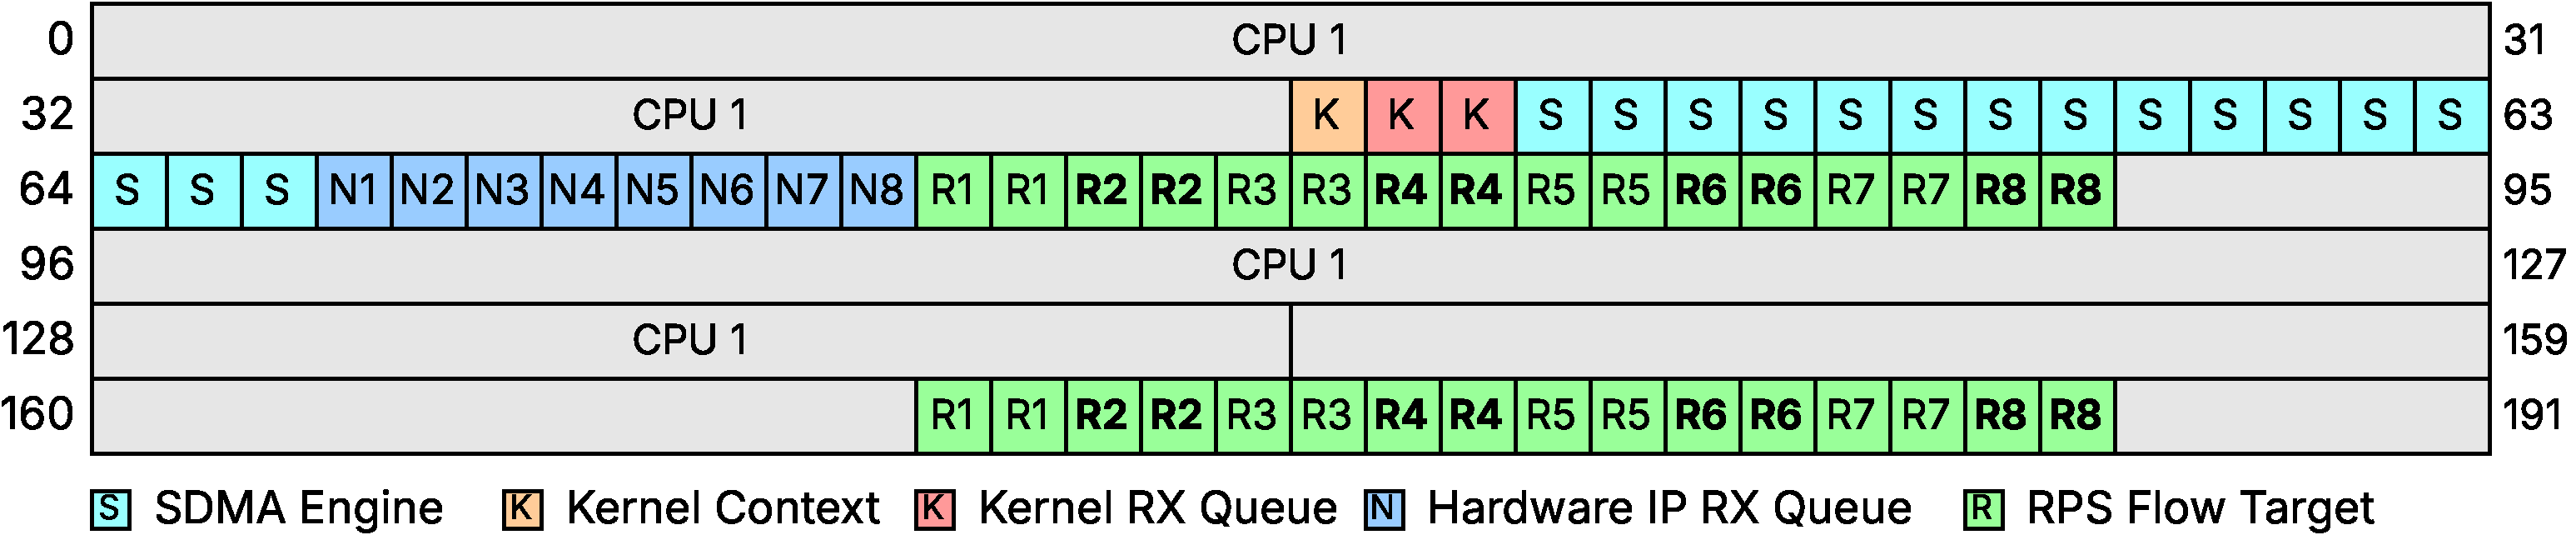
\includegraphics[width=\linewidth]{assets/network/rps/RPS-Single-NUMA.pdf}
    \caption{Single-\acs{NUMA}-Node \acs{RPS} Configuration}
    \label{fig:rps-single-numa}
\end{figure}

The unrestricted \ac{RPS} flow placement is shown in~\cref{fig:rps-multi-numa}.
It has significantly more cores per hardware interrupt to work with, but could
potentially perform worse due to the latency and bandwidth constraints
introduced by the inter-\ac{NUMA}-node link.

\begin{figure}[H]
    \centering
    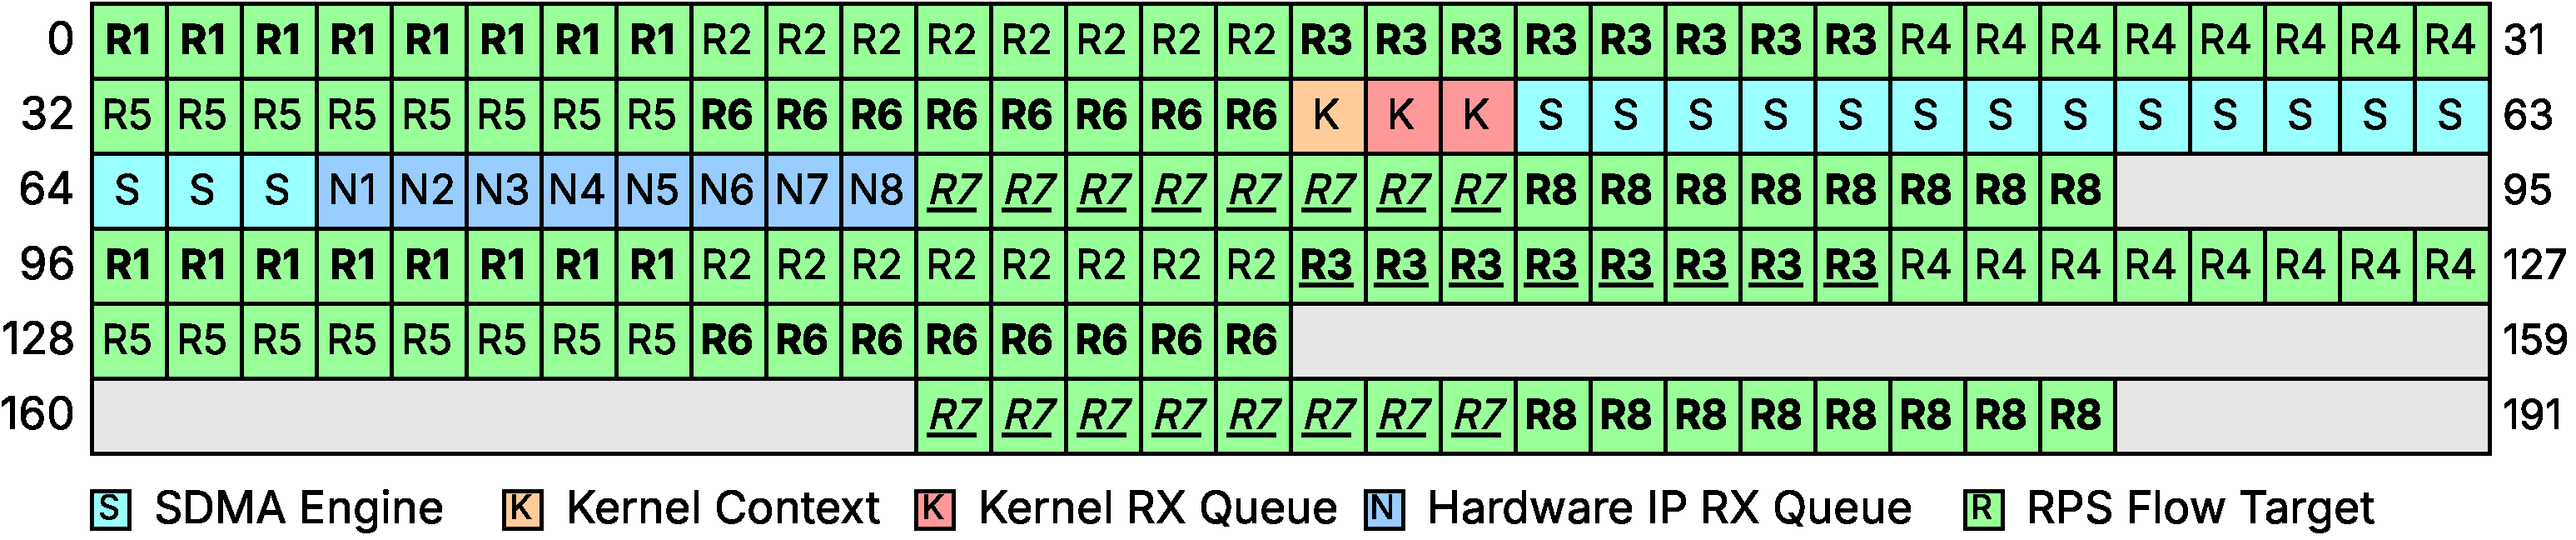
\includegraphics[width=\linewidth]{assets/network/rps/RPS-Multi-NUMA.pdf}
    \caption{Multi-\acs{NUMA}-Node \acs{RPS} Configuration}
    \label{fig:rps-multi-numa}
\end{figure}

% These optimizations were applied to the test nodes and initial testing was
% performed between two Omni-Path equipped test nodes
% (see~\cref{tbl:omnipath-system} for specifications). However, the observed
% performance results were poor.

\subsection{InfiniBand Optimizations}

InfiniBand supports Ceph's \ac{TCP/IP} traffic through its \ac{IPoIB} protocol. While all optimizations as shown in~\cref{tbl:nic-offload} for InfiniBand network adapters were enabled on the tested nodes, the \ac{MTU} was restricted to a maximum of 4000 bytes in order to preserve compatibility with existing infrastructure, such as storage servers and network switches. \Cref{tbl:infiniband-parameters} details the tuned system configuration applied to the test nodes, which were equipped with 200 Gbit/s NVIDIA ConnectX-6 adapters operating in InfiniBand mode.

\begin{table}[h]
\centering
\begin{tabular}{ll}
\hline
\textbf{Parameter}                      & \textbf{Value} \\
\hline
\ac{MTU}                                & 4000 \\
\ac{RPS}                                & Disabled \\
\texttt{irqbalance}                     & Enabled \\
\ac{THP}                                & Always \\
\ac{CPU} Scaling Governor               & Performance \\
\hline
\textbf{Kernel Parameter}               & \textbf{Value} \\
\hline
\texttt{iommu}                          & \texttt{pt} (Passthrough) \\
\texttt{ib\_ipoib.recv\_queue\_size}    & 8192 \\
\texttt{ib\_ipoib.send\_queue\_size}    & 8192 \\
\hline
\textbf{Sysctl Parameter}               & \textbf{Value} \\
\hline
\texttt{net.ipv4.tcp\_rmem}             & 16384 131072 16777216 \\
\texttt{net.ipv4.tcp\_wmem}             & 16384 16384 16777216 \\
\texttt{net.ipv4.rmem\_max}             & 16777216 \\
\texttt{net.ipv4.wmem\_max}             & 16777216 \\
\texttt{net.core.somaxconn}             & 2048 \\
\texttt{net.ipv4.tcp\_mtu\_probing}     & 1 \\
\texttt{net.core.netdev\_max\_backlog}  & 250000 \\


\hline
\end{tabular}
\caption{Configured Parameters for InfiniBand}
\label{tbl:infiniband-parameters}
\end{table}

Manual tuning of software interrupt handling, i.e., \ac{RPS}, was not considered necessary. In contrast to Omni-Path's capabilities, the InfiniBand network adapters supported hardware receive hashing/flow steering with 64 dedicated queues each for send and receive operations, compared to the 8 supported by Omni-Path.

\subsection{Benchmarking Goals}

The benchmarking methodology developed for this thesis is designed for the evaluation of the Ceph file system across diverse cluster configurations in order to assess its suitability for \ac{HPC} applications. To that end, we have deployed and evaluated two classes of Ceph clusters:

\begin{itemize}
    \item A simulated production environment (see~\cref{sec:production-deployment}), deployed with \texttt{cephadm}
    \item Custom in-memory deployments (see~\cref{sec:custom-deployment}), deployed with the Cuttlefish deployment tool developed for this thesis
\end{itemize}

In the production deployment, our benchmarking objectives are primarily qualitative and architectural evaluations. This deployment does not focus on peak performance measurements, as the constraints of the production deployment are controlled such that they are not expected to exceed Ceph's architectural capabilities. Instead, we have evaluated the orchestration process using \texttt{cephadm}, as well as analyzed potential deviations between theoretical performance models controlled by our performance throttling process and the observed behaviour of the cluster.

The in-memory deployment focuses primarily on quantitative stress testing in order to isolate Ceph's architectural performance limitations. These benchmarks are designed to evaluate Ceph's performance and scalability at various levels under high-load conditions, eliminating external compounding factors where possible. For instance, physical storage media such as hard drives and \acp{SSD} can have complex and potentially non-deterministic performance characteristics; using memory-backed \acp{OSD} eliminates disk performance as a source of potential performance bottlenecks. This methodology allows for an evaluation focused primarily on software overhead of the various layers of the Ceph file system, such as \ac{RADOS} and \ac{CephFS}, although other limiting factors such as memory and network bandwidth remain. 

\ac{IOR} and mdtest benchmark configurations were repeated 3 and 5 times respectively to account for random network jitter and other sources of variance. The higher repetition count for mdtest was chosen due to the higher observed variance in metadata operations compared to \ac{IOR}'s throughput measurements. Unless stated otherwise, the reported results are the mean across repetitions.

\subsubsection{Performance Testing}

Performance was evaluated through performance metrics obtained via two of its primary interfaces: the \ac{RADOS} object storage layer and \ac{CephFS}.

\ac{RADOS} performance benchmarks were used to establish a fundamental performance baseline, as it serves as the underlying storage method for all higher-level Ceph services, such as \ac{CephFS}, \ac{RBD}, and \ac{RGW}. As such, these measurements represent a theoretical \enquote{upper bound} of the cluster's throughput and \ac{I/O} capabilities at the lowest abstraction level.

The evaluation additionally includes \ac{CephFS} to assess performance in real-world deployments, such as the hosting of users' home directories or a high-performance scratch file system. In these scenarios, the overhead introduced by the implementation of a \ac{POSIX} compliant file system and its associated functionality is of particular concern. We have placed particular emphasis on metadata performance, as the \ac{MDS} daemons can represent a potential bottleneck, and common workloads such as the creation of Python virtual environments or compilation of software packages produce uniquely high-frequency bursts of small file \ac{I/O}.

A comparative analysis of \ac{RADOS} and \ac{CephFS} results with the same cluster configuration allows for the quantification of the overhead introduced specifically by the \ac{CephFS} file system abstraction layer.

\subsection{Benchmark Implementation}

\subsubsection{Modifications to \acs{IOR} and mdtest}
\label{sec:modifications-to-ior-mdtest}

During initial testing, bugs and limitations in \ac{CephFS} functionality within \ac{IOR} and mdtest were discovered and patched. The following components within the \ac{CephFS} backend were modified.

\begin{itemize}
    \item Addition of \texttt{mknod} and \texttt{rename} functionality, enabling the mdtest mknod folder creation and directory renaming tests
    \item Fix for the \texttt{CEPHFS\_StatFS} function to return correct index node utilization
\end{itemize}

These fixes enable full mdtest functionality on the \ac{CephFS} backend. Note
that the \ac{RADOS} backend, being an object store, does not provide a file
system structure to be tested. Therefore, \ac{RADOS} can only be tested with
\ac{IOR}.

In addition, the outputs provided by \ac{IOR} and mdtest are insufficient for
debugging, as they report only that operations have failed without exposing
additional details, such as error codes. This lack of information made issues
such as incorrect permissions or missing folders difficult to identify. The
programs were modified to emit detailed information on failure to address this
limitation. However, it does not affect the system's functionality and exists
purely as a debugging aid.

\subsubsection{Benchmarking Container Creation}

The Ceph image does not contain \ac{IOR} or mdtest on its own, and not all of
its dependencies were straightforward to install on Rocky Linux 8. This was
primarily due to the older software versions available in the package
repositories. Therefore, these were compiled from source on top of the existing
upstream Ceph container with a Dockerfile (see~\cref{appendix:ior-mdtest-dockerfile}).

The build script performs the following:

\begin{itemize}
    \item Installs the development headers and links \ac{IOR}/mdtest to the Ceph 
libraries, ensuring a version match with the containers on the server side.
    \item Installs Open \ac{MPI} to allow for communication between \ac{IOR} tasks.
    \item Enables the optional support for \acs{CephFS} and \acs{RADOS} within \ac{IOR}.
    \item Patches \ac{IOR}/mdtest to add the functionality specified in~\cref{sec:modifications-to-ior-mdtest}
\end{itemize}

Since the Docker build process outputs a Docker image, conversion into
Apptainer's native \ac{SIF} format is required. Apptainer provides functionality
to perform this conversion natively, however, there were some permission issues
experienced when building on top of the existing Ceph image. In order to fix
this, a simple shim script was created to run an Apptainer \texttt{-{}-fix-perms}
pass on the container image, which fixed issues experienced with running dnf in
the containers during debugging. The script is shown in~\cref{lst:sif-shim-fix-perms}.

\lstinputlisting[
    caption={\acs{SIF} Conversion Shim},
    label={lst:sif-shim-fix-perms},
    frame=single,
    breaklines=true
]{assets/cuttlefish/build_ior.sh}

The output container, \texttt{cf-bench-ior.sif}, is used specifically for
benchmarking. The unmodified Ceph container image is used for the daemons.

\subsubsection{Performance Scaling}

In order to evaluate and narrow down possible sources of performance bottlenecks, we will run performance tests using different combinations of clients and nodes. For instance, if a single node with 64 tasks performs worse than two nodes with 32 tasks each, it is possible that this is not a server-side bottleneck, but rather a client-side one, e.g., a compute or network bandwidth limitation.

To that end, a custom benchmarking script was developed which automates the running of various \ac{IOR} and mdtest configurations. The system shares some core components with the deployment system, such as the the Slurm interface, in order to determine the available nodes. The benchmarks are performed on the cluster based on the user's request and node allocation, and are saved to a database for further processing. The workflow is shown in~\cref{fig:cuttlefish-benchmark-flowchart}.

\begin{figure}[htbp]
    \centering
    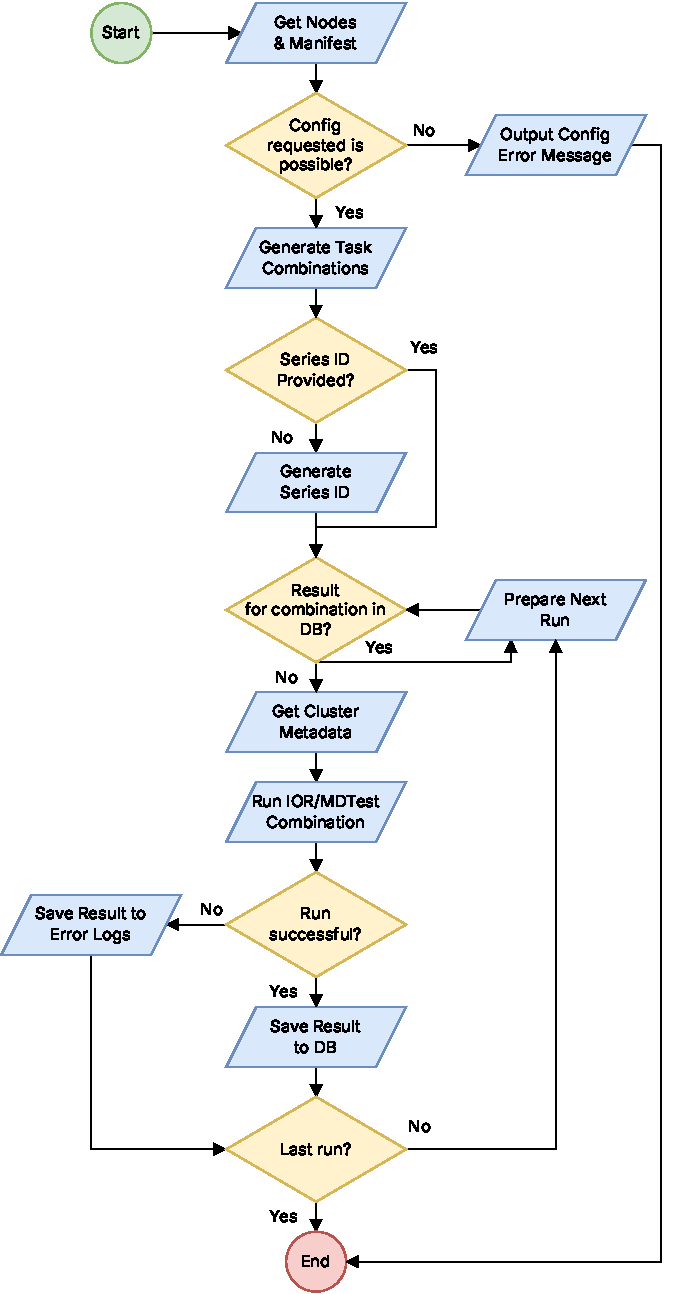
\includegraphics[width=0.7\linewidth]{assets/cuttlefish/benchmark_flowchart.pdf}
    \caption{Benchmarking Process Flowchart}
    \label{fig:cuttlefish-benchmark-flowchart}
\end{figure}

\subsubsection{Layout}

Two node types were tested: one with InfiniBand networking and one with
Omni-Path networking. All node types were running Rocky Linux 8.10 with the
kernel version 4.18.0-553.89.1.el8\_10.x86\_64.

The 16 InfiniBand test nodes were equipped with the hardware shown in
\cref{tbl:infiniband-system}.

\begin{table}[H]
\centering
\begin{tabular}{|ll|}
\hline
\textbf{Component} & \textbf{Specification} \\
\hline
CPU        & 2$\times$ AMD EPYC 7513 (32C/64T per CPU) \\
RAM        & 512 GB \\
Networking & 200 Gbps InfiniBand (NVIDIA ConnectX-6) \\
\hline
\end{tabular}
\caption{InfiniBand Test System Hardware}
\label{tbl:infiniband-system}
\end{table}

The Omni-Path nodes were equipped as shown in \cref{tbl:omnipath-system}.

\begin{table}[H]
\centering
\begin{tabular}{|ll|}
\hline
\textbf{Component} & \textbf{Specification} \\
\hline
CPU        & 2$\times$ Intel Xeon Platinum 8468 (48C/96T per CPU) \\
RAM        & 256 GB \\
Networking & 100 Gbps Omni-Path (Intel HFI100) \\
\hline
\end{tabular}
\caption{Omni-Path Test System Hardware}
\label{tbl:omnipath-system}
\end{table}

For all of the test systems, individual \acp{OSD} used the Memstore backend with
dynamic sizing, as described in~\cref{sec:ceph-autoconfig}. Due to the limited
number of available nodes, monitors are co-located with other daemon types on
the same node (e.g., \ac{MDS} daemons and \acp{OSD}).

\subsection{Data Collection}
\label{sec:data-collection}

By default, \ac{IOR} and mdtest emit human-readable data. They can also be
configured to output machine-readable data; \ac{IOR} can output \ac{JSON}
formatted data, while mdtest can output \ac{CSV} formatted data. However, some
challenges were faced when programmatically parsing the data:

\begin{itemize}
    \item Both \ac{IOR} and mdtest do not provide a formally specified data schema for their outputs, which complicates the inspection of output data.
    \item Units for bandwidth metrics in \ac{IOR} are expressed interchangeably in kilobytes and megabytes.
    \item The use of case is inconsistent throughout the output. For example, individual tests have the key \texttt{TestID}, while the test parameters have the key \texttt{testID}.
    \item Summary statistics are not directly associated with performed tests, complicating the attribution of summaries to test results for analysis.
\end{itemize}

In order to allow for easier result aggregation as well as more efficient storage of test results, data pass through a three-step process consisting of parsing, normalization, and database storage.

\subsubsection{\acs{IOR} Result Parsing}

Pydantic is used to parse \ac{IOR} results from the result \ac{JSON} data directly through conversion of field names and normalization of units. A snippet is shown in~\cref{lst:ior-result-pydantic} for a single \ac{IOR} result. Additional functions and Pydantic models are used for unit conversion and to cover the rest of the \ac{IOR} output, although they are not shown here.

\lstinputlisting[
    caption={[\acs{IOR} Result Pydantic Model]Pydantic model for the results gathered from a single \acs{IOR} repetition. Units are normalized to bytes per second, types are strongly defined, and validation of these types are performed by Pydantic. Keys use consistent snake-case throughout all models, regardless of the input case of the \acs{IOR}/mdtest data.},
    label={lst:ior-result-pydantic},
    frame=single,
    breaklines=true,
    language=python
]{assets/ior/ior_result.py}


\subsubsection{MDTest Result Parsing}

The \ac{CSV}-formatted results from mdtest cannot be parsed directly by Pydantic. Therefore, the fields are first read by the Python \texttt{csv} module, and the corresponding Pydantic models are generated using a conversion function. As opposed to \ac{IOR}, mdtest does not provide details such as the number of nodes or tasks, and therefore these must be provided separately in order for these metrics to be tracked. As the benchmarking script controls the instantiation of the mdtest runs and has the required information, this is passed through to the mdtest result parser, part of which is shown in~\cref{lst:mdtest-parser}.

\lstinputlisting[
    caption={[mdtest Result Parsing Logic]Snippet of code used to convert raw \acs{CSV} data output by mdtest into Pydantic mdtest models.},
    label={lst:mdtest-parser},
    frame=single,
    breaklines=true,
    language=python
]{assets/ior/mdtest_parser.py}

\subsubsection{Data Storage}

Once raw data have been converted into the exchange format, i.e., the Pydantic
models, they are normalized before being saved to a SQLite database. This
provides more flexibility when aggregating results due to the fact that all data
are saved in a single location and do not have to, for example, be manually read
from multiple output files. This is also more efficient for large numbers of
results, as the processing of text data (i.e., \ac{JSON}/\ac{CSV} outputs) must
only be performed once during the conversion step before being stored in an
efficient database-native format.

\begin{figure}[H]
    \centering
    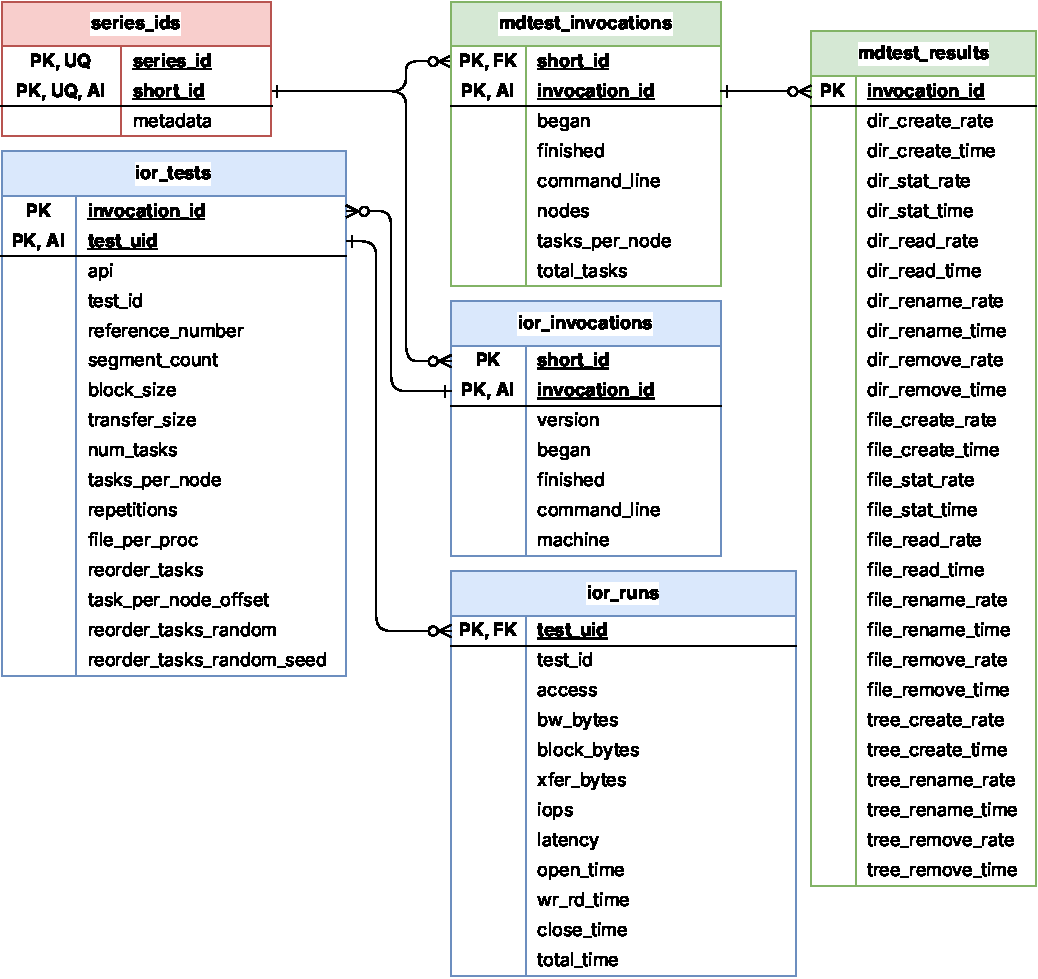
\includegraphics[width=\linewidth]{assets/cuttlefish/result-db-erd.pdf}
    \caption[Result Database ER Diagram]{\ac{ER} diagram of the result database, parsed from \acs{JSON} and \acs{CSV} data produced by \ac{IOR} and mdtest.}
    \label{fig:result-db-erd}
\end{figure}

\pagebreak

% In order to evaluate Ceph's performance characteristics, a benchmarking script
% runs multiple iterations of the \ac{IOR} benchmark with varied benchmark settings,
% numbers of client nodes and processes per node. To mimic a real-world
% deployment, the Ceph daemons and client nodes will be placed on separate
% machines. 

